\documentclass[14pt]{extarticle}

% file's preambule

% Если вы работаете не в XeLaTeX, то сами разбирайтесь =)

% connect packages
%%%%%%%%%%%%%%%%%%%%%%%%%%%%%%%%%%%%%%%%%%%%%%%%%%%%%%%%%%%%%%%%%%%%%%
%\usepackage[T2A]{fontenc}                   %!? закрепляет внутреннюю кодировку LaTeX
%\usepackage[utf8]{inputenc}                 %!  закрепляет кодировку utf8
\usepackage{fontspec}                        % Шрифты
\usepackage{indentfirst}                    %   добавить indent перед первым параграфом
\setlength{\parindent}{1.27cm}
\usepackage{polyglossia}                     % Русский язык
\setdefaultlanguage{russian}
\setmainfont[Ligatures=TeX]{Times New Roman}
\newfontfamily\cyrillicfont{Times New Roman}[Script=Cyrillic]
%\usepackage[english,russian]{babel}         %!  подключает русский и английский
\usepackage{amsmath}                        %!  |
\usepackage{amssymb,textcomp, esvect,esint} %!  |важно для формул 
\usepackage{geometry}                       %!  отступ от граней
\geometry{verbose,a4paper,tmargin=2cm,bmargin=2cm,lmargin=3cm,rmargin=1cm}
\usepackage{amsfonts}                       %!  математические шрифты
\usepackage{amsthm}                         %!  newtheorem и их сквозная нумерация
\usepackage{graphicx}                       %?  графическое изменение текста
\usepackage{soulutf8}% Поддержка переносоустойчивых подчёркиваний и зачёркиваний
\usepackage{enumitem}                       %!  задание макета перечня.
%\usepackage[unicode, pdftex]{hyperref}      %!  оглавление для панели навигации по PDF-документу + гиперссылки
\usepackage{setspace}                       % Межстроковые интервалы
\onehalfspacing
\usepackage{booktabs}                       %!  добавляет книжные линии в таблицы
%\usepackage{hypcap}                         %?  адресация на картинку, а не на подпись к ней
\usepackage{abraces}                        %?  фигурные скобки сверху или снизу текста
\usepackage{caption}                        %-  позволяет корректировать caption 
\DeclareCaptionLabelSeparator{dash}{ - }
\captionsetup[table]{labelformat=simple, labelsep=dash, justification=raggedleft,
singlelinecheck=off}
\captionsetup[figure]{labelformat=simple, labelsep=dash}
\usepackage{multirow}                       %   объединение ячеек в таблицах
\usepackage{longtable}
\usepackage{pifont}                         %!  нужен для крестика
\usepackage{cancel}                         %!  аутентичное перечеркивание текста
\usepackage{ulem}                           %!  перечеркивание текста
\usepackage{tikz}                           %!  высокоуровневые рисунки (кружочек)
\usepackage{titling}                        %-  автоматическое заглавие 
\usepackage{titlesec}  % нормальные заголовки секций
\titleformat{\section}
{\normalfont\large\bfseries\filcenter}{}{1em}{}
\titleformat{\subsection}
  {\normalfont\normalsize\bfseries}{\thesubsection.}{5pt}{}
\titleformat{\subsubsection}
  {\normalfont\normalsize\bfseries}{\thesubsubsection.}{5pt}{}
\titleformat{\paragraph}
  {\normalfont\normalsize\bfseries}{\theparagraph}{5pt}{}

\usepackage{ragged2e} % Для выравнивания текста по ширине
\justifying

%\renewcommand{\thesubsubsection}{\alph{subsubsection}}
\usepackage{blindtext}                      %-  слепой текст
\usepackage{fancyhdr}                       %   добавить верхний и нижний колонтитул
\usepackage{mathptmx}

\usepackage{import}                         %|
\usepackage{xifthen}                        %|
\usepackage{pdfpages}                       %|
%\usepackage{transparent}                    %| вставка ink figures
\usepackage{rotating}
\usepackage{array} % Картиночки в таблицы
%%%%%%%% Алгоритмы
\usepackage{float}
\usepackage{algorithm}
\usepackage{algpseudocode}
%%%%%%%%%%%%%%%

\usepackage{listings} % Для языков программирования 
\usepackage{xcolor}
\lstset {
    language=C++,
    backgroundcolor=\color{black!5}, % set backgroundcolor
    basicstyle=\footnotesize,% basic font setting
}

\usepackage{lmodern}

\colorlet{comment}{green!50!black}
\colorlet{cppcomment}{teal}
\colorlet{symb}{blue!50!black}
\colorlet{number}{violet}

\newcommand*{\textcolorsymb}{\textcolor{symb}}

\definecolor{backcolour}{rgb}{0.95,0.95,0.92}
\definecolor{black_red}{rgb}{0.54, 0, 0}

\lstdefinestyle{cpp}{%
  language=C++,
  columns=flexible,
  basewidth=.5em,  
  tabsize=2,
  basicstyle=\footnotesize,
  backgroundcolor=\color{backcolour},
  showspaces=false,
  showstringspaces=false,
  commentstyle={\itshape\color{comment}\let\textcolorsymb\relax},
  keywordstyle=\bfseries\color{black_red},
  morecomment={[l][\itshape\color{cppcomment}\let\textcolorsymb\relax]//},
  literate=%
    {\{}{\textcolorsymb{\{}}1
    {\}}{\textcolorsymb{\}}}1
    {(}{\textcolorsymb{(}}1
    {)}{\textcolorsymb{)}}1
    {;}{\textcolorsymb{;}}1
    {=}{\textcolorsymb{=}}1
    {<}{\textcolorsymb{<}}1
    {>}{\textcolorsymb{>}}1
    {!}{\textcolorsymb{!}}1
    {\&}{\textcolorsymb{\&}}1 
    {|}{\textcolorsymb{|}}1
    {?}{\textcolorsymb{?}}1
    {:}{\textcolorsymb{:}}1
    {+}{\textcolorsymb{+}}1
    {-}{\textcolorsymb{-}}1
    {,}{\textcolorsymb{,}}1
    {\%}{\textcolorsymb{\%}}1
    {\^}{\textcolorsymb{\textasciicircum}}1
    {~}{\textcolorsymb{\textasciitilde}}1
    %% {/}{\textcolorsymb{/}}1
    %% {*}{\textcolorsymb{*}}1
    % 2 (optionally)
    {==}{\textcolorsymb{==}}2
    {>=}{\textcolorsymb{=>}}2
    {<=}{\textcolorsymb{<=}}2
    {!=}{\textcolorsymb{!=}}2
    {+=}{\textcolorsymb{+=}}2
    {-=}{\textcolorsymb{-=}}2
    {*=}{\textcolorsymb{*=}}2
    {/=}{\textcolorsymb{/=}}2
    {\%=}{\textcolorsymb{\%=}}2
    {\&\&}{\textcolorsymb{\&\&}}2
    {||}{\textcolorsymb{||}}2
    {++}{\textcolorsymb{++}}2
    {--}{\textcolorsymb{--}}2
    {>>}{\textcolorsymb{>\kern0pt>}}2
    {<<}{\textcolorsymb{<\kern0pt<}}2
    {::}{\textcolorsymb{::}}2
    % 3 (optionally)
    {>>=}{\textcolorsymb{>\kern0pt>=}}3
    {<<=}{\textcolorsymb{<\kern0pt<=}}3
    % Remove byte order mark
    {^^ef^^bb^^bf}{}0
}
\lstnewenvironment{cpp}{\lstset{style=cpp}}{}
\lstset{style=cpp}
  


%%%%%%%%%%%%%%%%%%%%%%%%%%%%%%%%%%%%%%%%%%%%%%%%%%%%%%%%%%%%%%%%%%%%%%


%%%%%%%%%%%%%%%%%% ВСТАВКА РИСУНКО ИЗ INKSCAPE %%%%%%%%%%%%%%%%%%%%%%%
\newcommand{\incfig}[1]{%
    \def\svgwidth{\columnwidth}
    \import{./figures/}{#1.pdf_tex}
}

%%%%%%%%%%%%%%%%%%%%%%%%%%%%%%%%%%%%%%%%%%%%%%%%%%%%%%%%%%%%%%%%%%%%%%


\newenvironment{itemize*}
{
    \begin{itemize}
        \setlength{\itemsep}{1pt}
        \setlength{\parskip}{1pt}}
    {\end{itemize}
}

\newenvironment{enumerate*}
{
    \begin{enumerate}
        \setlength{\itemsep}{1pt}
        \setlength{\parskip}{1pt}}
    {\end{enumerate}
}

%%%%%%%%%%%%%%%%%%%%%%%%%%%%%%%%%%%%%%%%%%%%%%%%%%%%%%%%%%%%%%%%%%%%%%


\begin{document}

\includepdf{titul_third.pdf}
\newpage
\tableofcontents
\newpage
\section{Первое задание}
\subsection{Постановка задачи}
Оценить зависимость времени выполнения алгоритма простой
сортировки на массиве, заполненном случайными числами (в соответствии с
персональным вариантом).

Вариант 2. (сортировка простого обмена или пузырьком)
\subsection{Алгоритм сортировки}
Схема алгоритма представлена на рисунке \ref{fig:first_alg_scheme}.

\begin{figure}[htpb]
  \centering
  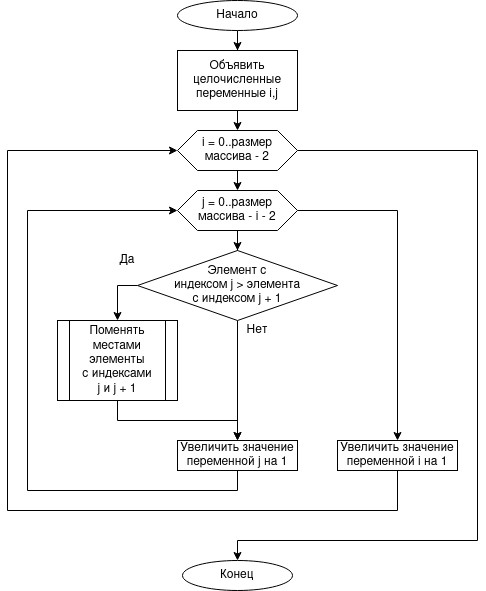
\includegraphics[width=0.7\textwidth]{pictures/first_task.png}
  \caption{Блок-схема первого алгоритма}
  \label{fig:first_alg_scheme}
\end{figure}
\newpage

Результаты тестирования алгоритма на заполненном с клавиатуры массиве
(рис. \ref{fig:test1_alg1}), а также на случайно заполненном массиве
(рис. \ref{fig:test2_alg1} и \ref{fig:test3_alg1}).

\begin{figure}[htpb]
  \centering
  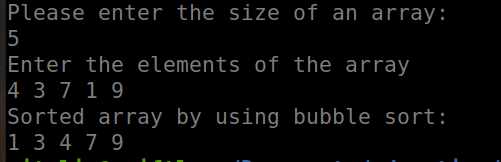
\includegraphics[width=0.7\textwidth]{pictures/test1_alg1.png}
  \caption{Результаты тестирования алгоритма на введенном пользователем массиве}
  \label{fig:test1_alg1}
\end{figure}

\begin{figure}[htpb]
  \centering
  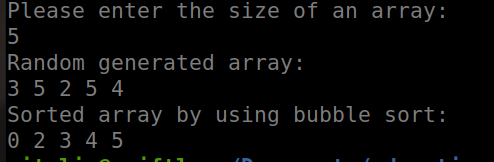
\includegraphics[width=0.7\textwidth]{pictures/test2_alg1.png}
  \caption{Результаты тестирования алгоритма на случайном массиве размером 5}
  \label{fig:test2_alg1}
\end{figure}

\begin{figure}[htpb]
  \centering
  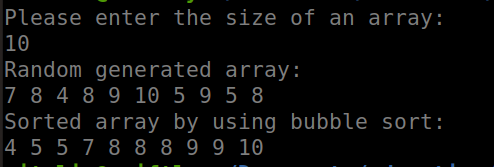
\includegraphics[width=0.7\textwidth]{pictures/test3_alg1.png}
  \caption{Результаты тестирования алгоритма на случайном массиве размером 10}
  \label{fig:test3_alg1}
\end{figure}

\newpage
\subsection{Оценка функции роста выполнения алгоритма сортировки пузырьком}
Определим теоретическую сложность алгоритма при помощи таблицы
операторов.

\begin{table}[htpb]
  \centering
  \caption{Подсчет количества операторов в алгоритме сортировки простого обмена}
  \label{tab:first_alg_speed}
  \begin{tabular}{|c|c|c|c|}
    \hline
    \parbox[m]{2cm}{\centering Номер \\ оператора}
    & Оператор
    & \parbox[m]{2cm}{\centering Время выполнения \\ одного оператора}
    & \parbox[m]{2cm}{\centering Кол-во выполнений \\ оператора в строке}
    \\ \hline
    1 & int n = v.size(); & C1 & 1 раз
    \\ \hline
    2 & \parbox[m]{4cm}{\centering for (int i = 0;\\ i < n-1; ++i) \{ }
      & C2 & n раз
    \\ \hline
      3 &\parbox[m]{4cm}{\centering for (int j = 0;\\ j < n - i - 1;
         ++j) \{ } & C3 & n(n-1) раз
    \\ \hline
        4 & if (v[j] > v[j+1]) \{  & C4 & n(n-1) - 1 раз
    \\ \hline
    5 & std::swap(v[j], v[j+1]);\}\}\} & C5 & n(n-1) - 1 раз
    \\ \hline
  \end{tabular}
\end{table}

Из таблицы \ref{tab:first_alg_speed} получим функцию роста выполнения алгоритма
сортировки простого обмена. Пусть $T(n)$ - время выполнения алгоритма, зависящее
от  $n$. Тогда
 
\[
  T(n) = C_1 + C_2\cdot n + C_3\cdot (n^2-n) + C_4\cdot (n^2-n-1)
  + C_5\cdot (n^2-n-1)
.\] 

После упрощения получаем
\[
  T(n) = C_1 + C_2\cdot n + C_3 \cdot n^2 - C_3\cdot n + C_4\cdot n^2
  - C_4\cdot n - C_4 + C_5\cdot n^2 - C_5\cdot n - C_5
.\] 
Подведя подобные, получаем
\[
  T(n) = An^2+Bn+C
.\] 
Оставляя справа только доминирующую функцию, получаем порядок роста
$T(n) = O(n^2)$, где  $n$ - размер массива.
\subsection{Результаты выполнения сортировки}
Представлены на рисунках \ref{fig:alg_speed1}, \ref{fig:alg_speed2}
и на таблице \ref{tab:testing1}.

\begin{figure}[htpb]
  \centering
  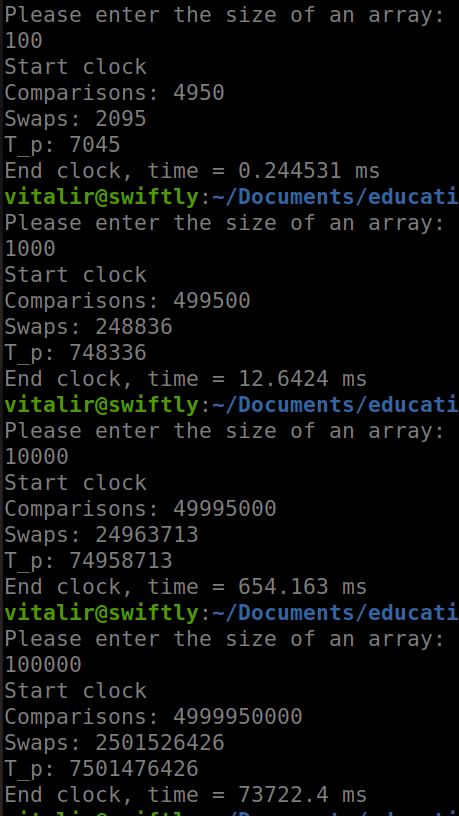
\includegraphics[width=0.5\textwidth]{pictures/alg1_speed1.png}
  \caption{Результаты выполнения программы задания 1, 1 часть}
  \label{fig:alg_speed1}
\end{figure}

\begin{figure}[htpb]
  \centering
  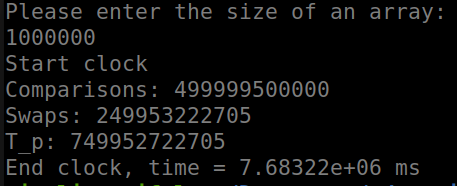
\includegraphics[width=0.5\textwidth]{pictures/alg1_speed2.png}
  \caption{Результаты выполнения программы задания 1, 2 часть}
  \label{fig:alg_speed2}
\end{figure}


\begin{table}[htpb]
  \centering
  \caption{Сводная таблица тестирования сортировки пузырьком}
  \label{tab:testing1}
  \begin{tabular}{|c|c|c|c|}
    \hline
    n & $T(n)$ & $T_\textup Т=f(C+M)$ &
    $T_\textup п=C_\textup ф+M_\textup ф$
    \\ \hline
    100
    & 0.244351 мс
    & \multirow{5}*{\centering $O(n^2)$} 
    & 7045
    \\ \cline{1-2}\cline{4-4}
    1000
    & 12.6424 мс
    &
    & 748336
    \\ \cline{1-2}\cline{4-4}
    10000
    & 654.163 мс
    &
    & 74958713
    \\ \cline{1-2}\cline{4-4}
    100000
    & 73722.4 мс
    &
    & 7501476426
    \\ \cline{1-2}\cline{4-4}
    1000000
    & 7683220 мс
    &
    & 749952722705
    \\ \hline
  \end{tabular}
\end{table}
\newpage
\subsection{Код алгоритма и основной программы}
Алгоритм сортировки простым обменом представлен на рисунке \ref{fig:alg1_code_sort}.
\begin{figure}[htpb]
  \centering
  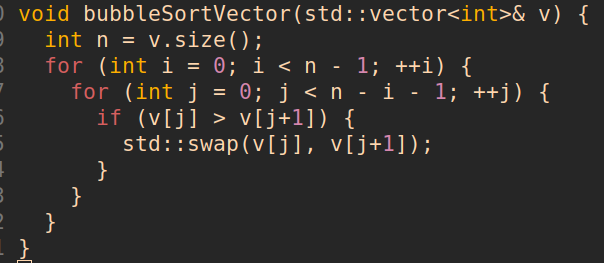
\includegraphics[width=0.8\textwidth]{pictures/alg1_code_sort.png}
  \caption{Код функции сортировка простым обменом}
  \label{fig:alg1_code_sort}
\end{figure}
\newpage
Для отладки были реализованы функции генерации случайного массива, класс для
замерения времени и отдельная функция сортировки простым обменом со встроенным
подсчетом практической сложности (представлены, соотвественно, на рисунках
\ref{fig:alg1_code_random}, \ref{fig:alg1_code_timer}, \ref{fig:alg1_code_sort_debug}).

\begin{figure}[htpb]
  \centering
  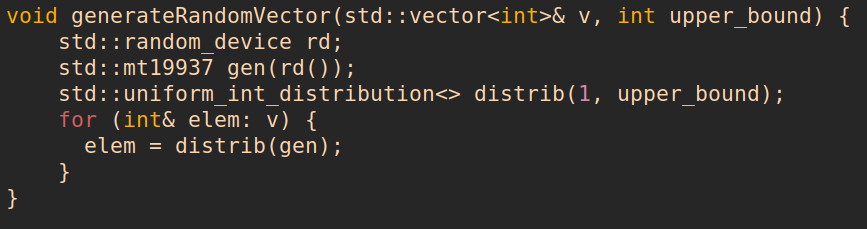
\includegraphics[width=0.8\textwidth]{pictures/alg1_code_random.png}
  \caption{Код функции генерации случайного массива}
  \label{fig:alg1_code_random}
\end{figure}

\begin{figure}[htpb]
  \centering
  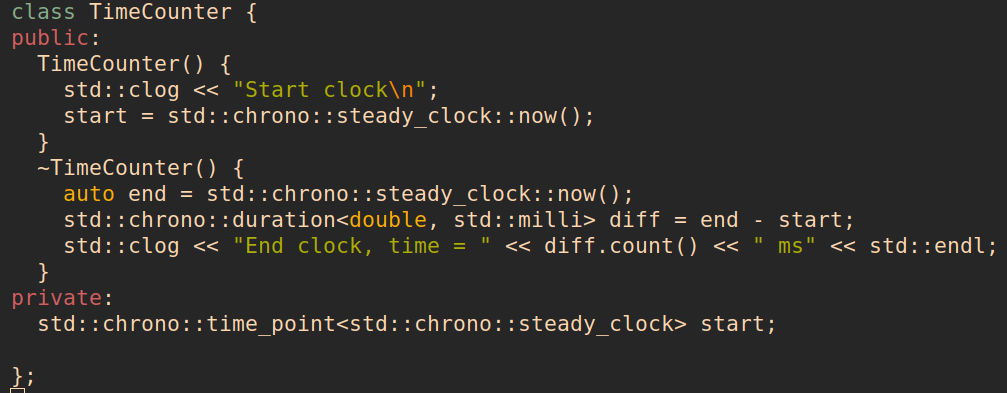
\includegraphics[width=0.8\textwidth]{pictures/alg1_code_timer.png}
  \caption{Код класса для замера времени выполнения}
  \label{fig:alg1_code_timer}
\end{figure}

\begin{figure}[htpb]
  \centering
  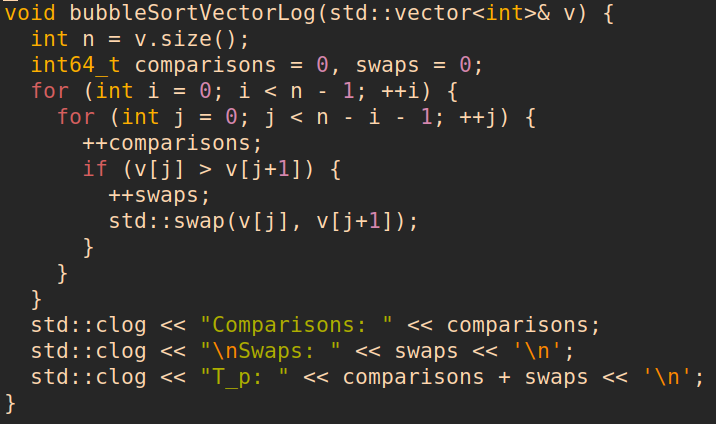
\includegraphics[width=0.8\textwidth]{pictures/alg1_code_sort_debug.png}
  \caption{Код функции сортировки простым обменом с подсчетом операций}
  \label{fig:alg1_code_sort_debug}
\end{figure}

\newpage
Главная функция программы представлена на рисунке \ref{fig:alg1_code_main}.
\begin{figure}[htpb]
  \centering
  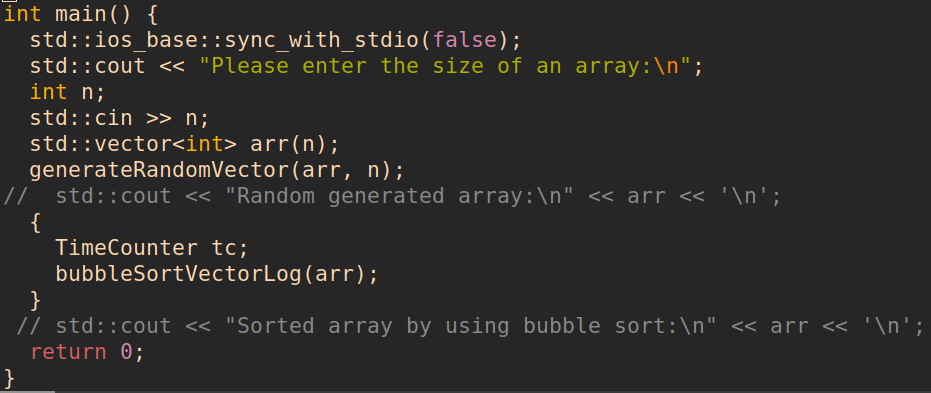
\includegraphics[width=0.8\textwidth]{pictures/alg1_code_main.png}
  \caption{Главная функция программы задания 1}
  \label{fig:alg1_code_main}
\end{figure}

\subsection{Графики зависимостей теоретической и практической сложности}
Для вычисления зависимости практической вычислительной сложности
алгоритма от размера n массива можно воспользоваться калькулятором методов
регрессии для аппроксимации функции одной переменной. Наименьшая
ошибка аппроксимации приходится на степенную модель регрессии с
показателем, приблизительно равным 2.
\newpage
\begin{figure}[htpb]
  \centering
  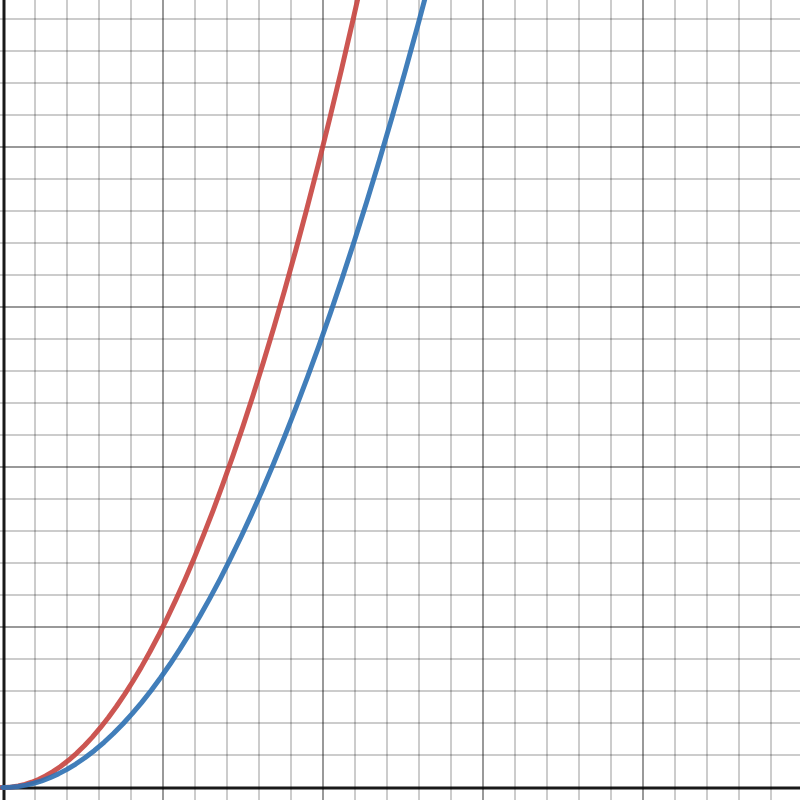
\includegraphics[width=0.6\textwidth]{pictures/desmos_first.png}
  \caption{График зависимости теоретической и практической сложности алгоритма
  сортировки простым обменом}
  \label{fig:graph_1}
\end{figure}
На рисунке \ref{fig:graph_1} показаны графики теоретической зависимости
$f(n) = n^2$ (красным)
и практической зависимости $g(n) = 0.7035x^{2.0055}$ (синим) вычислительной сложности алгоритма
от размера массива.
\subsection{Анализ результатов}
Из графика видно, что эмпирически полученные данные не
противоречат теоретическим расчетам вычислительной сложности
алгоритма: сложность алгоритма имеет квадратичную зависимость от
размера входных данных.

\section{Задание 2}
\subsection{Постановка задачи}
Оценить вычислительную сложность алгоритма простой сортировки (в
соответствии с персональным вариантом) в наилучшем и наихудшем
случаях.

Вариант 2.
\newpage
\subsection{Результаты тестирования на массиве, отсортированном строго по возрастанию}

\begin{figure}[htpb]
  \centering
  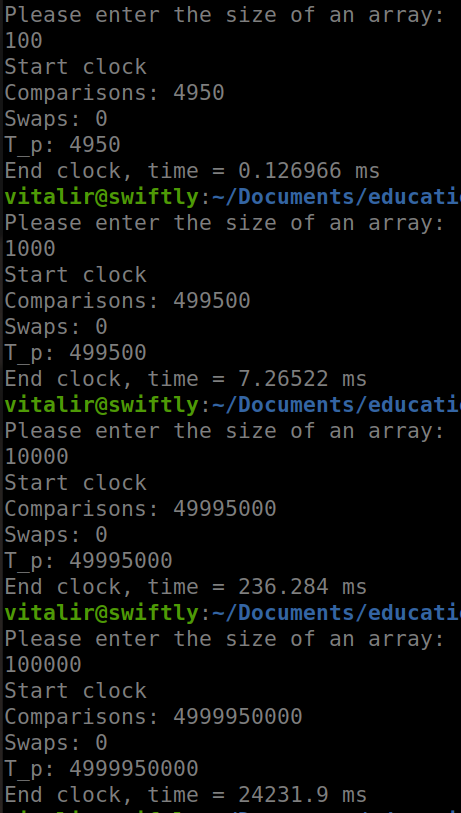
\includegraphics[width=0.5\textwidth]{pictures/alg2_speed1.png}
  \caption{Результаты выполнения программы задания 2, лучший случай, 1 часть}
  \label{fig:alg2_speed1_best}
\end{figure}

\begin{figure}[htpb]
  \centering
  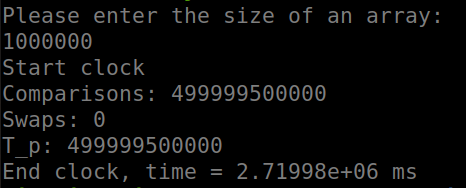
\includegraphics[width=0.5\textwidth]{pictures/alg2_speed2.png}
  \caption{Результаты выполнения программы задания 2, лучший случай, 2 часть}
  \label{fig:alg2_speed2_best}
\end{figure}


\begin{table}[htpb]
  \centering
  \caption{Сводная таблица тестирования в лучшем случае}
  \label{tab:testing2}
  \begin{tabular}{|c|c|c|c|}
    \hline
    n & $T(n)$ & $T_\textup Т=f(C+M)$ &
    $T_\textup п=C_\textup ф+M_\textup ф$
    \\ \hline
    100
    & 0.126966 мс
    & \multirow{5}*{\centering $O(n^2)$} 
    & 4950
    \\ \cline{1-2}\cline{4-4}
    1000
    & 7.26552 мс
    &
    & 499500
    \\ \cline{1-2}\cline{4-4}
    10000
    & 236.284 мс
    &
    & 49995000
    \\ \cline{1-2}\cline{4-4}
    100000
    & 24231.9 мс
    &
    & 4999950000
    \\ \cline{1-2}\cline{4-4}
    1000000
    & 7683220 мс
    &
    & 749952722705
    \\ \hline
  \end{tabular}
\end{table}
\newpage
Отсюда $T(n) = \frac{n^2-n}{2}$.
\newpage
\subsection{Результаты тестирования на массиве, отсортированном строго по убыванию}

\begin{figure}[htpb]
  \centering
  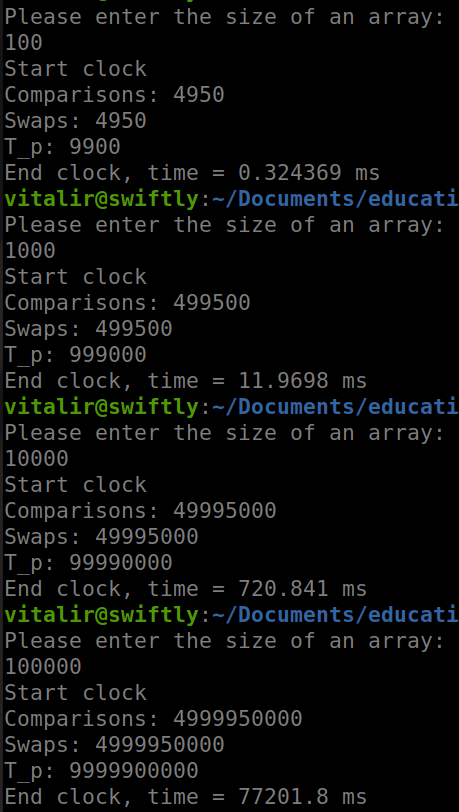
\includegraphics[width=0.5\textwidth]{pictures/alg2_speed1_bad.png}
  \caption{Результаты выполнения программы задания 2, худший случай, 1 часть}
  \label{fig:alg2_speed1_bad}
\end{figure}

\begin{figure}[htpb]
  \centering
  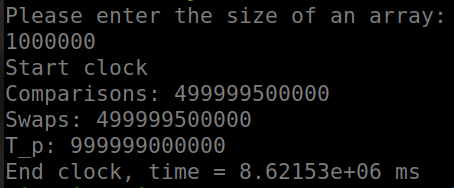
\includegraphics[width=0.5\textwidth]{pictures/alg2_speed2_bad.png}
  \caption{Результаты выполнения программы задания 2, худший случай, 2 часть}
  \label{fig:alg2_speed2_bad}
\end{figure}

\begin{table}[htpb]
  \centering
  \caption{Сводная таблица тестирования в худшем случае}
  \label{tab:testing_task2_bad}
  \begin{tabular}{|c|c|c|c|}
    \hline
    n & $T(n)$ & $T_\textup Т=f(C+M)$ &
    $T_\textup п=C_\textup ф+M_\textup ф$
    \\ \hline
    100
    & 0.324369 мс
    & \multirow{5}*{\centering $O(n^2)$} 
    & 9900
    \\ \cline{1-2}\cline{4-4}
    1000
    & 11.9698 мс
    &
    & 999000
    \\ \cline{1-2}\cline{4-4}
    10000
    & 720.841 мс
    &
    & 99990000
    \\ \cline{1-2}\cline{4-4}
    100000
    & 77201.8 мс
    &
    & 9999900000
    \\ \cline{1-2}\cline{4-4}
    1000000
    & 8621530 мс
    &
    & 999999000000
    \\ \hline
  \end{tabular}
\end{table}
\newpage
Отсюда $T(n) = n^2-n$.

\subsection{Код тестирующей программы}
Для тестирования лучших и худших случаев сортировки были созданы
функции для заполнения массива в порядке возрастания и убывания,
а также немного изменена главная функция программы (рис. \ref{fig:task2_code}).
\begin{figure}[htpb]
  \centering
  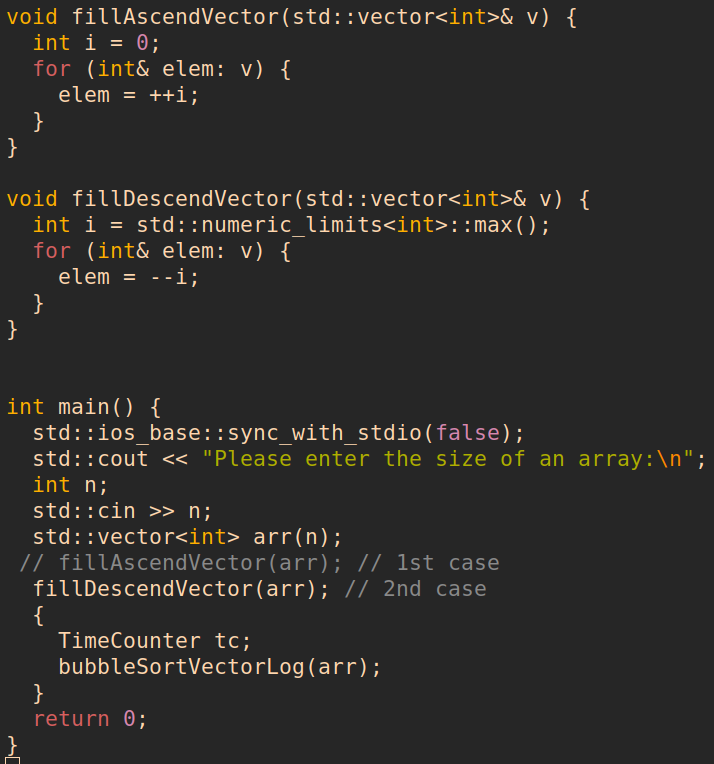
\includegraphics[width=0.6\textwidth]{pictures/second_task_code.png}
  \caption{Код программы задания 2}
  \label{fig:task2_code}
\end{figure}
\newpage
\subsection{График зависимости теоретической и практической
вычислительной сложности алгоритма для трех рассмотренных случаев}

\begin{figure}[htpb]
  \centering
  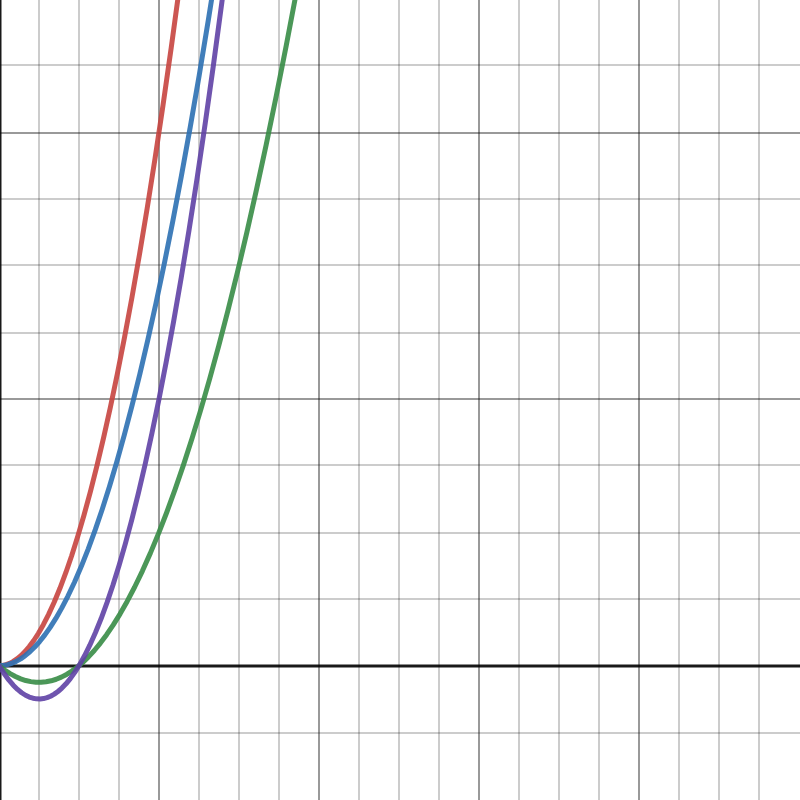
\includegraphics[width=0.6\textwidth]{pictures/desmos_second.png}
  \caption{Графики зависимостей вычислительной сложности сортировки пузырьком от n}
  \label{fig:graph_2}
\end{figure}

На рис. \ref{fig:graph_2} представлены графики зависимостей теоретической (красный) и
практической (синий для табл. \ref{tab:first_alg_speed},
зеленый для табл. \ref{tab:testing2} , темно-фиолетовый для табл. \ref{tab:testing_task2_bad})
вычислительных сложностей алгоритма. При этом квадратичная зависимость
для теоретической сложности сохраняется во всех рассмотренных случаев,
исходя из выведенных формул функции роста времени для худшего и лучшего
случаев. Графики практических сложностей для упорядоченного массива
являются квадратичными зависимостями с формулами $T(n) = \frac{n^2-n}{2}$
для лучшего случая и  $T(n) = n^2-n$ для худшего случая.

\subsection{Емкостная сложность алгоритма от $n$ }
Алгоритм сортировки методом простого обмена имеет линейную емкостную сложность
$O(n)$, т.к. в процессе сортировки обрабатывается только исходный массив размера n.
\subsection{Анализ результатов}
Установленная эмпирическим путем зависимость вычислительной
сложности алгоритма подтверждает найденную ранее теоретическую
сложность. Для лучшего случая в алгоритме количество операций сравнения
при увеличении размера массива в 10 раз увеличивается в 100, а операции
перестановки не выполняются совсем. Для худшего же случая сохраняется
квадратичная зависимость критических операций от размера массива.
\section{Задание 3}
\subsection{Постановка задачи}
Выполнить разработку алгоритма и программную реализацию
алгоритма задания 3. Сформировать таблицу в соответствии с форматом
таблицы 2 на тех же массивах, что и в задании 1. Выполнить сравнительный
анализ полученных результатов контрольных прогонов и построением
соответствующих графиков. Определить емкостную сложность алгоритма от
n.

Вариант 2 (сортировка простыми вставками)
\subsection{Алгоритм сортировки}
Схема алгоритма представлена на рисунке \ref{fig:second_alg_scheme}.

\begin{figure}[htpb]
  \centering
  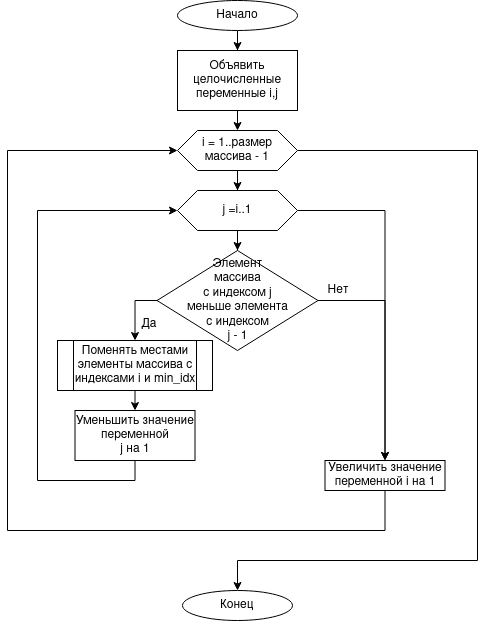
\includegraphics[width=0.7\textwidth]{pictures/task_3.png}
  \caption{Блок-схема второго алгоритма}
  \label{fig:second_alg_scheme}
\end{figure}
\newpage

\subsection{Оценка функции роста выполнения алгоритма сортировки вставками}
Определим теоретическую сложность алгоритма при помощи таблицы
операторов.

\begin{table}[htpb]
  \centering
  \caption{Подсчет количества операторов в алгоритме сортировки простых вставок}
  \label{tab:second_alg_speed}
  \begin{tabular}{|c|c|c|c|}
    \hline
    \parbox[m]{2cm}{\centering Номер \\ оператора}
    & Оператор
    & \parbox[m]{2cm}{\centering Время выполнения \\ одного оператора}
    & \parbox[m]{2cm}{\centering Кол-во выполнений \\ оператора в строке}
    \\ \hline
    1 & \parbox[m]{4cm}{\centering for (int i = 1;\\ i < n; ++i) \{ }
      & C1 & n раз
    \\ \hline
      2 & \parbox[m]{4cm}{\centering for (int j = i;\\ j > 0 \&\& v[j] < v[j-1]; --j) \{ }
        & C2 & n(n-1) раз
    \\ \hline
  3 & std::swap(v[j], v[j-1]);\}\} & C3 & n(n-1)-1 раз
    \\ \hline
  \end{tabular}
\end{table}

Из таблицы \ref{tab:second_alg_speed} получим функцию роста выполнения алгоритма
сортировки простыми вставками. Пусть $T(n)$ - время выполнения алгоритма, зависящее
от  $n$. Тогда
 
\[
  T(n) = C_1\cdot n + C_2\cdot (n^2-n) + C_3\cdot (n^2-n-1)
.\] 

После упрощения получаем
\[
  T(n) = C_1\cdot n + C_2\cdot n^2 - C_2 \cdot n + C_3\cdot n^2 - C_3\cdot n
  - C_3
.\] 
Подведя подобные, получаем
\[
  T(n) = An^2+Bn+C
.\] 
Оставляя справа только доминирующую функцию, получаем порядок роста
$T(n) = O(n^2)$, где  $n$ - размер массива.
\subsection{Результаты выполнения сортировки}
Для произвольного массива
\begin{figure}[htpb]
  \centering
  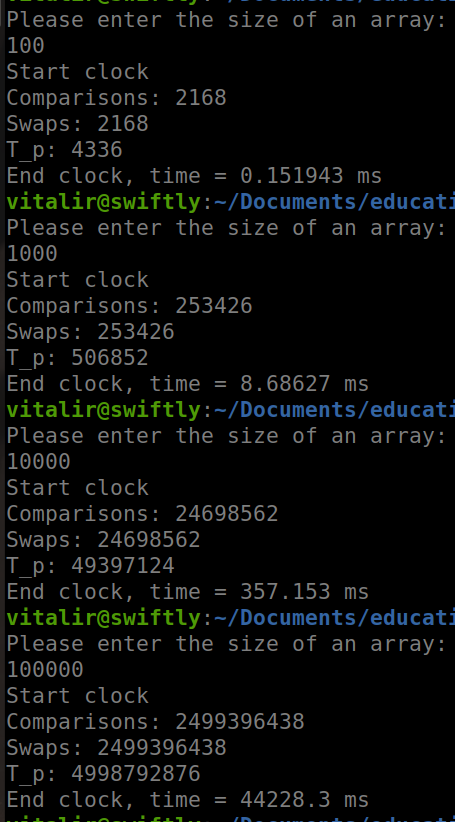
\includegraphics[width=0.5\textwidth]{pictures/alg3_speed1.png}
  \caption{Результаты выполнения программы задания 3, случайный массив, 1 часть}
  \label{fig:alg2_speed_general1}
\end{figure}

\begin{figure}[htpb]
  \centering
  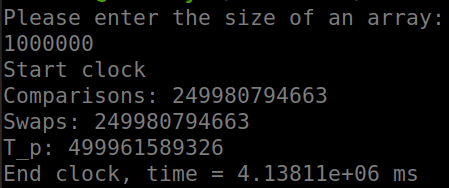
\includegraphics[width=0.5\textwidth]{pictures/alg3_speed2.png}
  \caption{Результаты выполнения программы задания 3, случайный массив, 2 часть}
  \label{fig:alg2_speed_general2}
\end{figure}


\begin{table}[htpb]
  \centering
  \caption{Сводная таблица тестирования сортировки вставками}
  \label{tab:testing_task3}
  \begin{tabular}{|c|c|c|c|}
    \hline
    n & $T(n)$ & $T_\textup Т=f(C+M)$ &
    $T_\textup п=C_\textup ф+M_\textup ф$
    \\ \hline
    100
    & 0.151943 мс
    & \multirow{5}*{\centering $O(n^2)$} 
    & 4336
    \\ \cline{1-2}\cline{4-4}
    1000
    & 8.68627 мс
    &
    & 506852
    \\ \cline{1-2}\cline{4-4}
    10000
    & 357.153 мс
    &
    & 49397124
    \\ \cline{1-2}\cline{4-4}
    100000
    & 44228.3 мс
    &
    & 4998792876
    \\ \cline{1-2}\cline{4-4}
    1000000
    & 4138110 мс
    &
    & 499961589326
    \\ \hline
  \end{tabular}
\end{table}

\subsection{Код программы}
\begin{figure}[htpb]
  \centering
  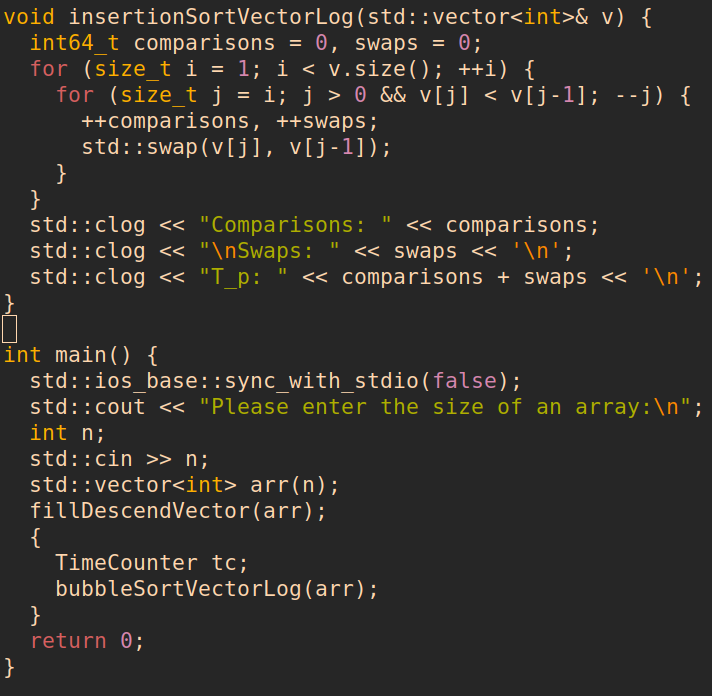
\includegraphics[width=0.6\textwidth]{pictures/alg3_code.png}
  \caption{Код программы тестирования сортировки вставками}
  \label{fig:alg3_code}
\end{figure}

Для тестирования программы был разработан код функции сортировки простыми вставками
с отладкой и немного изменен код главной функции (см. рис. \ref{fig:alg3_code}).
\subsection{График зависимости вычислительных сложностей для 2 случаев}
\begin{figure}[htpb]
  \centering
  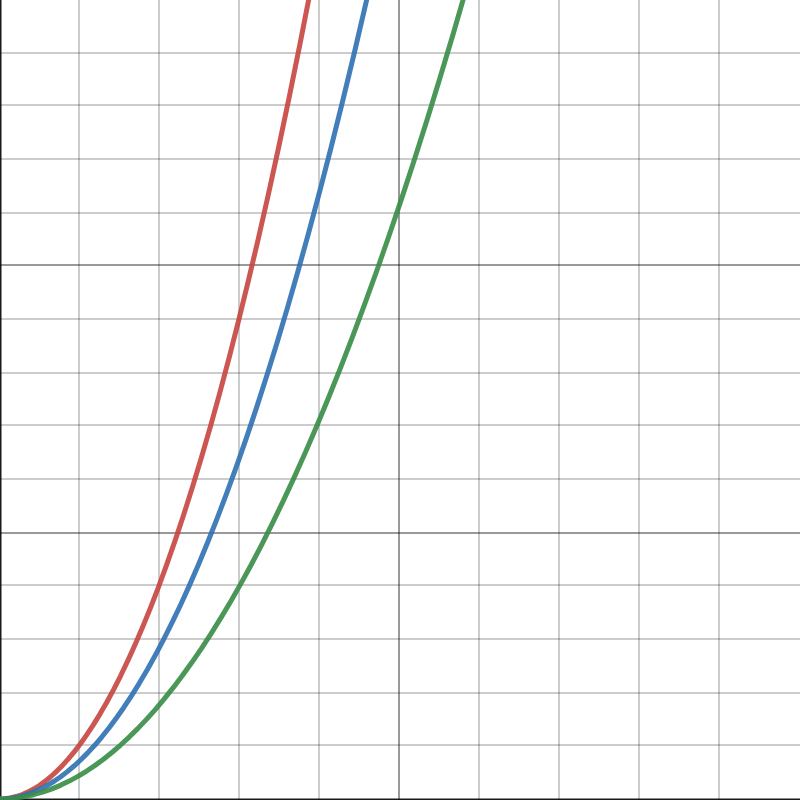
\includegraphics[width=0.6\textwidth]{pictures/desmos_third.png}
  \caption{Сравнение вычислительных сложностей сортировок пузырьком и вставкой}
  \label{fig:graph_3}
\end{figure}
На рис. \ref{fig:graph_3} отображена зависимость теоретической (синий) и практической
(красный для алгоритма простого обмена, зеленый для алгоритма простой вставки с
формулой
$y=0.4361^{2.0118}$).
вычислительных сложностей. Теоретическая сложность у
обоих алгоритмов квадратично зависит от размера массива.
\subsection{Определение эффективности алгоритма}
Эффективность алгоритма — это свойство алгоритма, которое связано с
вычислительными ресурсами, используемыми алгоритмом. Алгоритм считается
эффективным, если потребляемый им ресурс (или стоимость ресурса) являются
наиболее оптимальными. Оценка эффективности алгоритма состоит в определении
времени его выполнения и объема потребляемой им памяти. Алгоритм считается
эффективнее другого, если время его работы в наихудшем случае имеет более
низкий порядок роста.
\subsection{Сравнение эффективности двух алгоритмов из заданий 1 и 3}
Сравнивая алгоритмы в среднем, лучшем и худшем случаях, можно сделать вывыд,
что сортировка вставками работает быстрее сортировки пузырьком (по графикам
практических зависимостей,
а также в лучшем случае сортировка вставками имеет линейную зависимость, в отличии
от сортировки пузырьком).
\newpage
\section{Ответы на дополнительные вопросы}
\paragraph{Вопрос 7}
Примением условие Айверсона к алгоритму сортировки простого обмена,
для этого изменив код функции (см рис. \ref{fig:alg3_code_aiv}).
\begin{figure}[htpb]
  \centering
  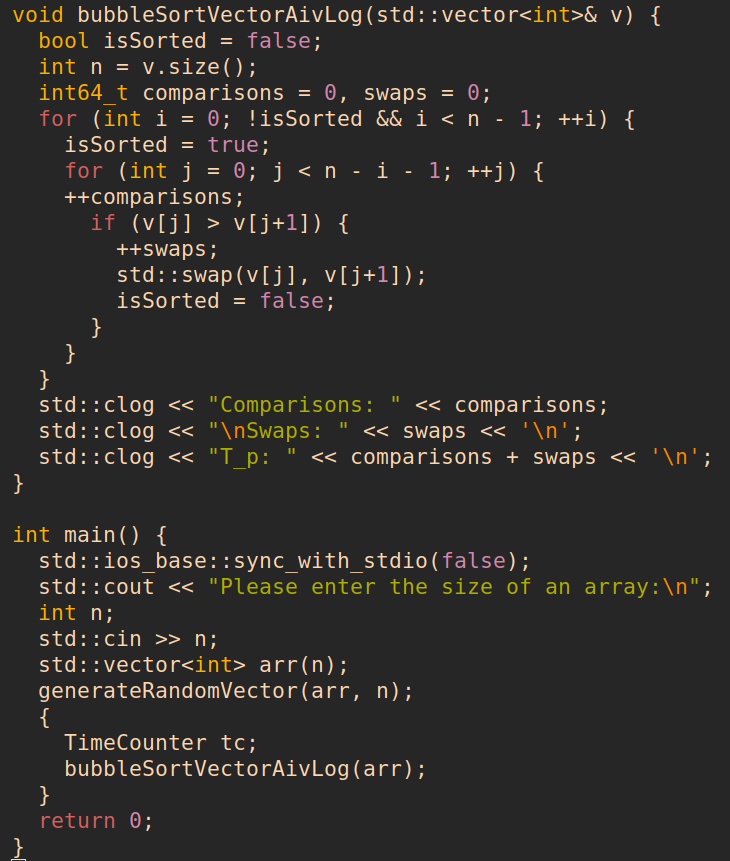
\includegraphics[width=0.6\textwidth]{pictures/alg3_code_aiv.png}
  \caption{Код измененного фрагмента программы сортировки пузырьком с использованием
  условия Айверсона}
  \label{fig:alg3_code_aiv}
\end{figure}

\newpage
\begin{figure}[htpb]
  \centering
  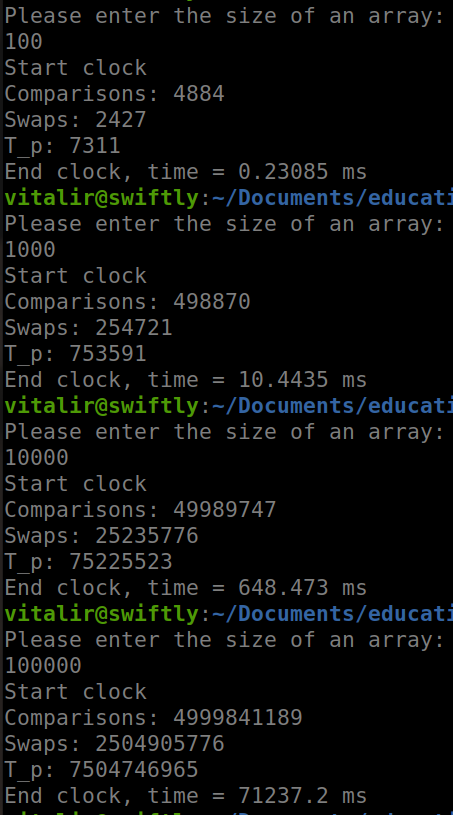
\includegraphics[width=0.4\textwidth]{pictures/alg1_aiv_speed1.png}
  \caption{Результаты выполнения программы вопроса 7, случайный массив, 1 часть}
  \label{fig:qs7_speed1}
\end{figure}

\begin{figure}[htpb]
  \centering
  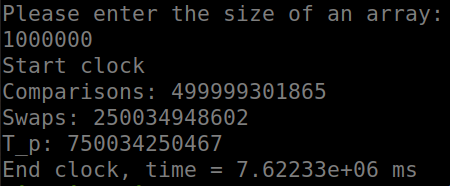
\includegraphics[width=0.5\textwidth]{pictures/alg1_aiv_speed2.png}
  \caption{Результаты выполнения программы вопроса 7, случайный массив, 2 часть}
  \label{fig:qs7_speed2}
\end{figure}

\newpage
\begin{table}[htpb]
  \centering
  \caption{Сводная таблица тестирования сортировки обмена с условием Айверсона}
  \label{tab:testing_aiv}
  \begin{tabular}{|c|c|c|c|}
    \hline
    n & $T(n)$ & $T_\textup Т=f(C+M)$ &
    $T_\textup п=C_\textup ф+M_\textup ф$
    \\ \hline
    100
    & 0.23085 мс
    & \multirow{5}*{\centering $O(n^2)$} 
    & 7311
    \\ \cline{1-2}\cline{4-4}
    1000
    & 10.4435 мс
    &
    & 753591
    \\ \cline{1-2}\cline{4-4}
    10000
    & 648.473 мс
    &
    & 75225523
    \\ \cline{1-2}\cline{4-4}
    100000
    & 71237.2 мс
    &
    & 7504746965
    \\ \cline{1-2}\cline{4-4}
    1000000
    & 7622330 мс
    &
    & 750034250467
    \\ \hline
  \end{tabular}
\end{table}


Сравнивая таблицы \ref{tab:first_alg_speed} и \ref{tab:testing_aiv}, можно сделать вывод, что условие Айверсона
особо не влияет на расчет эффективности алгоритма сортировки
простого обмена.
\paragraph{Вопрос 8}
Сортировка массива [5 6 1 2 3] с данными шагами является сортировкой
простой вставки, суть которой заключается в переборе массива, при котором на
каждом шаге элемент перемещается на свое конечное место, начиная с начала массива.
\paragraph{Вопрос 9}
В лучшем случае алгоритм имеет порядок
роста времени $O(n)$, в худшем $O(n^2)$ операций сравнения и перестановки. 
Емкостная сложность составляет $O(n)$, так как используется только один массив данных.
\newpage
\section{Выводы}
В ходе выполнения практической работы были изучены методы оценки времени
выполнения алгоритмов простых сортировок (сортировки пузырьком и
простыми вставками) на случайно заполненных массивах.
Данные алгоритмы были описаны на языке блок-схем, реализованы
на языке C++, была определена теоретическая сложность в наилучшем и
наихудшем случаях, выполнен прогон алгоритмов на тестовых данных для
среднего, наилучшего и наихудшего случаев, определена практическая
сложность алгоритмов. Из результатов тестирования, теоретические
предположения совпали с полученными эмпирически данными. Основываясь
на этих данных, алгоритм пузырьковой сортировки почти в два раза
менее эффективнее по времени чем алгоритм сортировки вставками.
\section{Список используемой литературы}
\begin{enumerate}
  \item Thomas H. Cormen, Clifford Stein и другие: Introduction to Algorithms, 3rd Edition.
    Сентябрь 2009. The MIT Press.
  \item B. Strousrup: A Tour of C++ (2nd Edition). Июль 2018. Addison-Wesley.
  \item Difference between bubblesort \& insertion sort~//~Pediaa \\~
    [Электронный ресурс]. URL:
    \\ https://pediaa.com/what-is-the-difference-between-bubble-sort-and-insertion-sort/\\
    (Дата обращения: 05.04.2021)
   \item Курс Algorithms, part 1 // Coursera [Электронный ресурс]. URL:
     \\ https://www.coursera.org/learn/algorithms-part1
     (Дата обращения: 05.04.2021)
\end{enumerate}
\end{document}
